\section{Introduction}

The domain of stream programs is important because it stands at the
intersection of trends in applications and architectures.  Stream
programming naturally represents applications such as audio, video,
digital signal processing, and data analysis; applications that are
increasingly prevalent as computing moves towards data-centric
applications and to the mobile and embedded space.  Also, by virtue of
their structure -- a graph of independent computational nodes (termed
{\it filters}) with explicit and regular communication -- stream
programs are a natural fit for exploiting coarse-grained parallelism
suitable for multicore architectures.  The interest in streaming
applications has spawned a number of streaming languages that target
the streaming domain, including StreamIt~\cite{streamitcc},
Brook~\cite{brook04}, Cg~\cite{cg03},
SPUR~\cite{spur05samos}, Spidle~\cite{spidle03}, Lime~\cite{lime10},
and SPL~\cite{spl09}.

In a stream program, each filter defines an atomic execution step that
repeats for many iterations; each execution step discards a number of
data items from the filter's input edge.  Often, a filter does not
discard all the data items that it read for the current execution
step, requiring these inspected (but not discarded) items for a future
iteration of the filter.  This type of filter is described as
performing a sliding window computation on its input. Sliding window
computations are prevalent in stream programs.  Examples of sliding
window computations include FIR filters; moving averages and
differences; error correcting codes; motion estimation; and network
packet inspection.  A recent study of a large streaming benchmark
suite written in the StreamIt programming language finds that 17 of
the 30 real-world benchmarks include at least one filter that performs
a sliding window computation~\cite{streamit-suite}.

A goal of stream programming is to directly expose to the software
layer the necessary information to enable automatic management of
coarse-grained parallelism.  Stream programs expose multiple forms of
parallelism; however, data parallelism is the most attractive.  Data
parallelism exists when a filter is stateless and can thus be
replicated.  Data parallelism provides load-balanced and limitless
parallelism (as long as input data is available).  A filter that is
stateful, and cannot be data-parallelized, becomes a limit to
parallelization scalability, as the work of that filter cannot be
divided; the most load-intensive stateful filter becomes a bottleneck.

Figure~\ref{fig:fir-nopeeking} shows how to implement a sliding window
FIR filter via state carried between iterations of a filter in the
form of a circular buffer.  This implementation is extremely difficult
for the compiler to analyze and reason about.  If the compiler cannot
precisely reason about the state of a filter, it will be prevented
from data-parallelizing the filter, and this state could represent the
parallelization bottleneck.  If a compiler cannot data-parallelize them,
sliding window computations would become the bottleneck in 11 of the
17 real-world benchmarks in the StreamIt Benchmark Suite that contain
sliding windows~\cite{streamit-suite}.

 Some programming languages (e.g., Brook, Lime,
StreamIt, and IBM SPL) go so far as to include idioms that directly
represent sliding window computation, allowing the programmer to
specify, for each filter, the size of the window and the number of
items discarded after an execution of the filter.
Figure~\ref{fig:fir-peeking} shows how language extensions of the
StreamIt programming language elegantly expose sliding windows for
compiler analysis and optimization.  The {\tt peek} and {\tt pop}
declarations of the {\tt work} function declare the number of items
inspected and the number of items dequeued, respectively, from the
 input edge for each firing of the filter.

This paper presents a compiler framework for data-parallelizing
filters that perform sliding window computations.  The framework is
enabled by languages that expose sliding windows so that the
properties of the sliding window can be calculated statically.
Data-parallelizing a filter is performed via a transformation termed
{\it fission} (verb form {\it fiss})~\cite{streamit-asplos}.  Fission
is the process of data-parallelizing a stateless filter by duplicating
the filter a certain number of ways, assigning duplicates to distinct
cores, and correctly distributed input data to and collecting output
data from the duplicates.  The duplicated filters are referred to as
{\it products}.  When a sliding window is present, fission is
accomplished by duplicating certain input items since they are
required by multiple products.  This duplication translates into
inter-core communication, a limiting factor for scalability when
targeting multicore architectures.

Previous approaches duplicate each input data item to all products,
with products ignoring (decimating) items that are not
needed~\cite{streamit-asplos}.  We will show that this strategy limits
scalability for multicores by requiring too much inter-core
communication.  In contrast, our strategy precisely routes each input
item to the minimal set of product filters that requires the item.
% Unlike previous work, our techniques are defined on
% multiple input and multiple output filters, removing the need to
% introduce synchronization filters that serialize data before and
% after the product filters.  

Our techniques operate on {\it static-rate} stream graphs, meaning
that the number of items produced, the number of items consumed, and
the number of items inspected by each filter can be determined
statically.  Because of this property, a steady-state schedule of
filter firings can be calculated that does not grow buffers and can be
executed indefinitely~\cite{lee87}.  Our techniques are conscious of
the spatial locality between producers and consumers.  Our framework
includes techniques that can determine when spatial locality can be
increased by altering the steady-state schedule.  When applicable, our
techniques can reduce the overall sharing (and thus inter-core
communication) requirement to below a threshold percent of the total
input communication for each sliding window filter that is
data-parallelized. 

\begin{figure}[t]
\centering
\subfigure[]{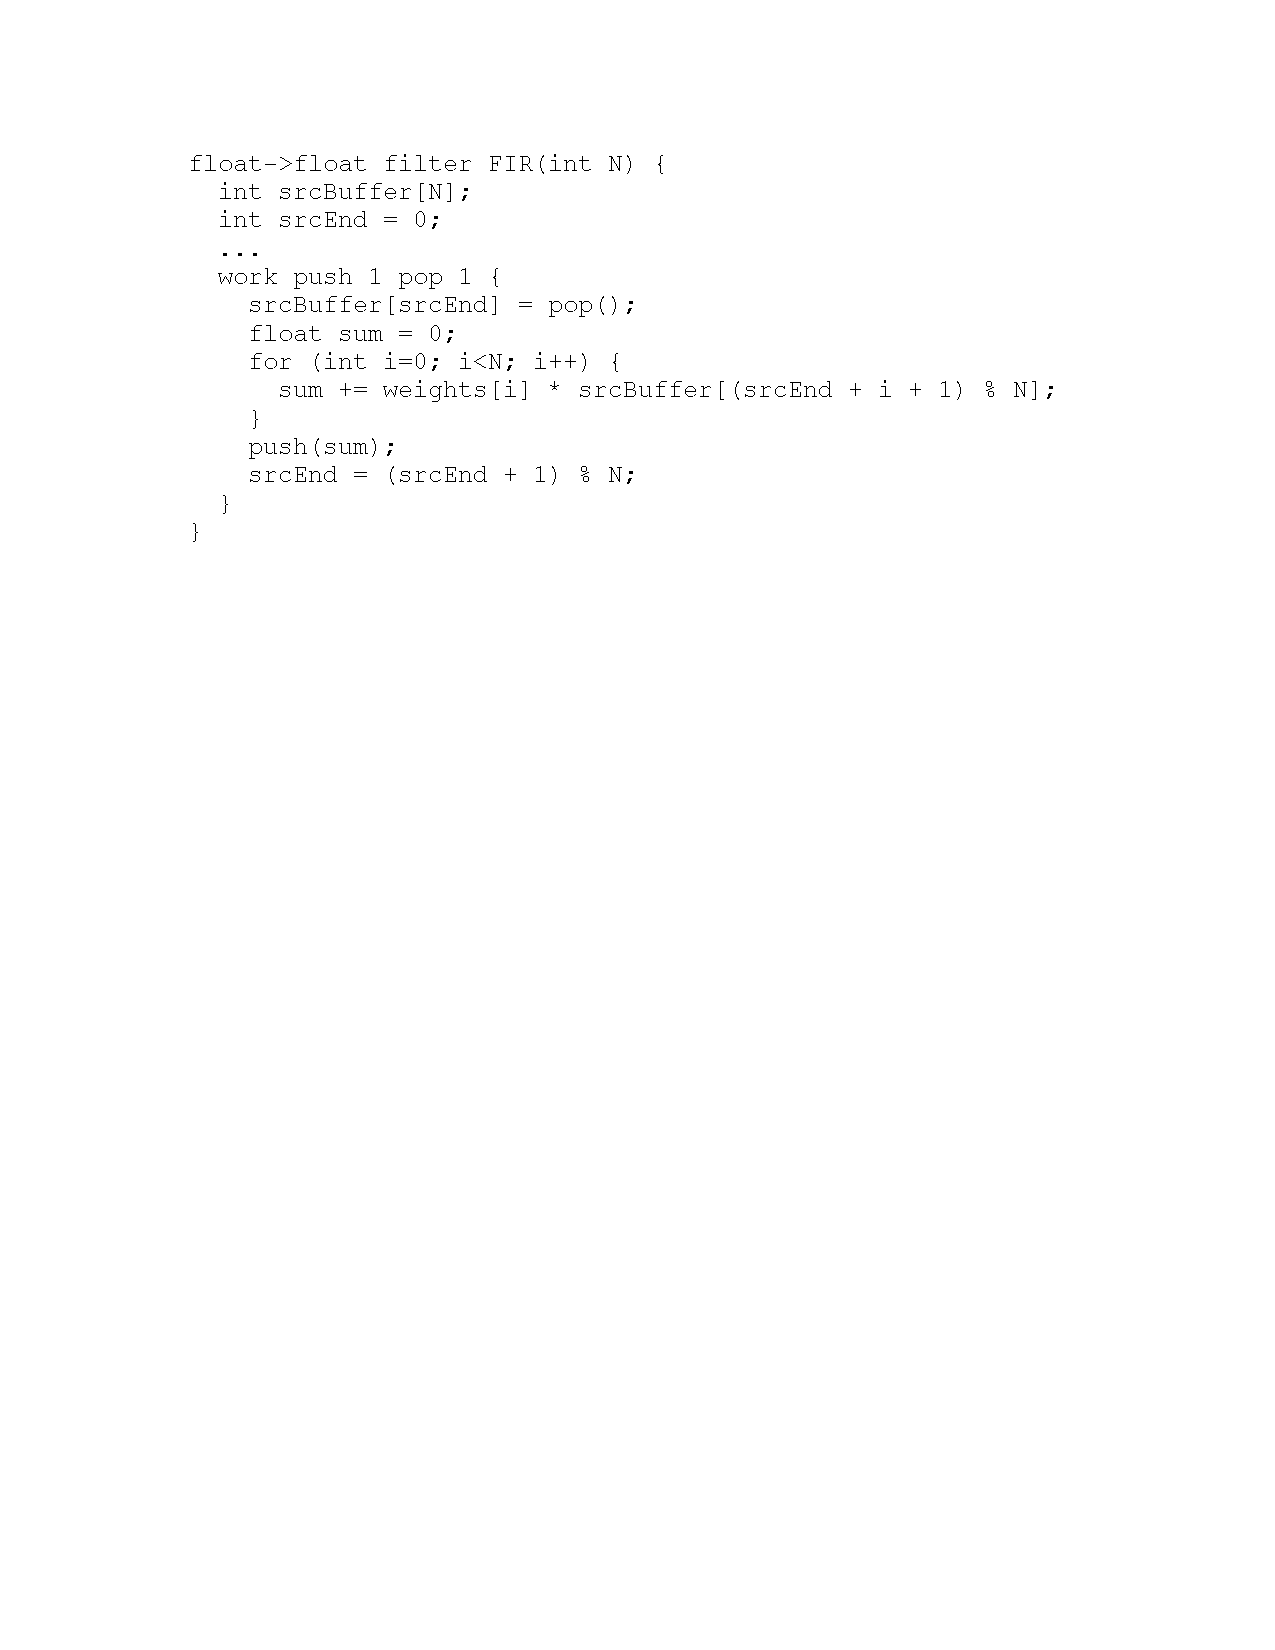
\includegraphics[width=3.3in]{figures/fir-nopeeking.pdf}\label{fig:fir-nopeeking}}
\subfigure[]{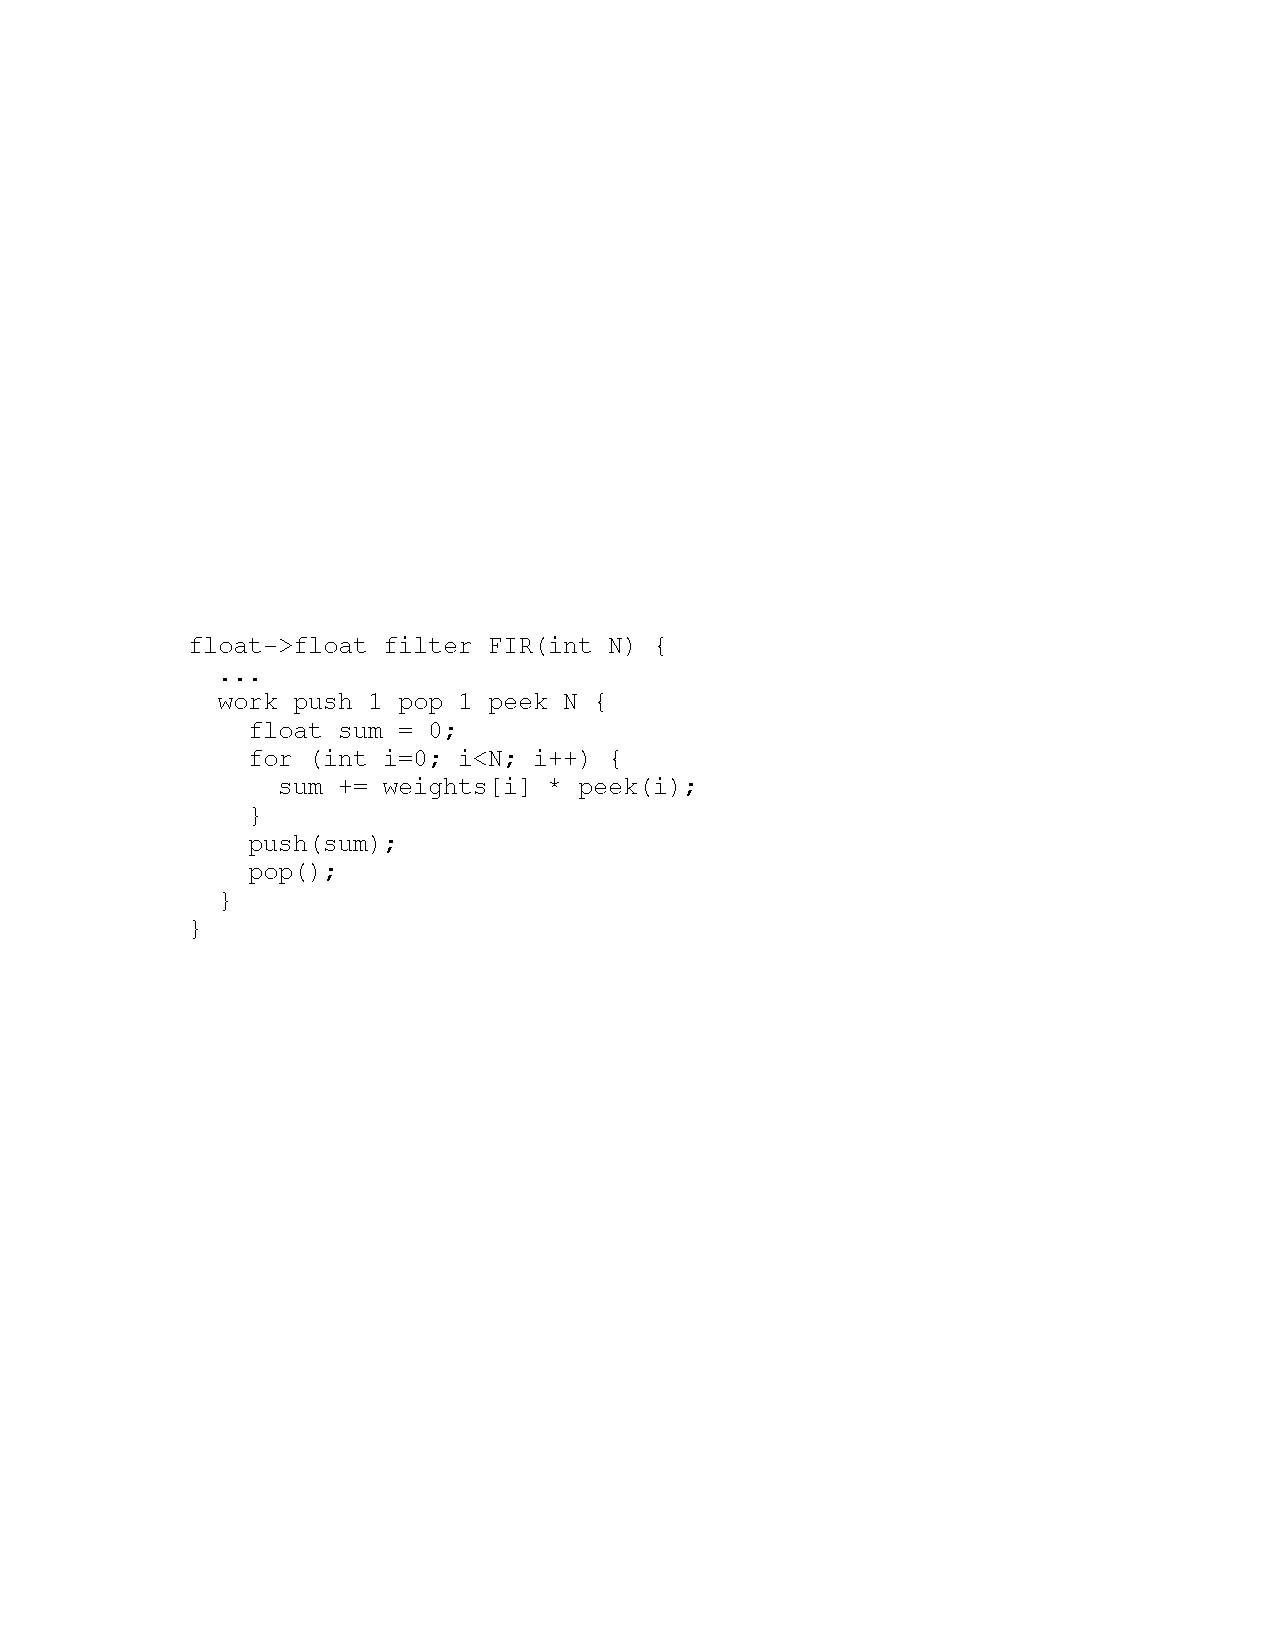
\includegraphics[width=3.3in]{figures/fir-peeking.pdf}\label{fig:fir-peeking}}
\caption[Two implementations of an FIR filter.]{\label{fig:fir-code}
  Two StreamIt implementations of an FIR filter:
   (a) the non-peeking version implemented via a
  stateful circular buffer; and (b) the peeking version. Only steady-state implementation is
  given.}
\vspace{-10pt}
\end{figure}

The framework presented is defined on an execution model that is
agnostic of source language.  For evaluation, we have implemented our
techniques in the context of the StreamIt compiler
infrastructure~\cite{gordon-asplos06}.  Our transformations are guided
by the parallelization management techniques presented
in~\cite{gordon-asplos06}.  We employ 3 real-world benchmarks that
include sliding window computation from the StreamIt Benchmark
Suite~\cite{streamit-suite}.  We demonstrate the effectiveness of our
techniques by comparing them to previously published techniques on two
multicore architectures: a 16-core SMP shared-memory multicore and the
64-core distributed-memory Tilera TILE64.  We show that our techniques
are required to achieve scalable parallelization on both
architectures, achieving a 6.7x mean speedup on the 16-core SMP and a
1.8x mean speedup on the 64-core TILE64 over a
previously published technique.

\subsection{Perspective on our Framework}

To appreciate the contributions of our framework, consider the
following.  In a translation to an imperative language, each filter is
wrapped in a scheduling loop that executes for the number of times
that the filter appears in the steady-state schedule. An array
implements the input edge of each filter.  All loops that represent
filters are then wrapped in an outer loop that executes until input
data is exhausted.  For sliding window filters, data items must be
saved across iterations of the outer steady-state loop employing
either a circular buffer or copy/shift operators, both of which are
non-affine.

Many traditional frameworks are able to parallelize the inner
scheduling loop of a sliding window filter within a single iteration
of the outer loop, and block executions to reduce communication of
shared data.  This corresponds to parallelizing and blocking a stencil
pattern across loop iterations.  However, we do not know of a
framework that will parallelize and block the inner scheduling loop
across iterations of the outer steady-state loop because, for sliding
window fliters, the inner loop's dependences across outer loop
iterations are non-affine.

Our techniques are able to parallelize and block the inner scheduling
loop across iterations of the outer steady-state loop in the presence
of non-affine dependences.  This capability enables a programmer to
write an application and its filters at a natural granularity that is 
independent of parallelization considerations.  The compiler
schedules filter executions and parallelizes at the appropriate
granularity to reduce inter-core communication.

% \subsection{Contributions}
% This paper makes the following contributions:
% \begin{itemize}
%   % \myitem{Motivation for Exposing Sliding Windows in Stream
%   %   Languages}: Without exposing sliding windows in the language, it
%   % requires heroic effort by the compiler to analyze the access patterns
%   % of such a filter. Without success, the compiler will not be able to
%   % data-parallelize these filters.  This will prevent robust 
%   % parallelization scalability for streaming applications.

%   \myitem{Generalized Fission of Sliding Window Filters}: We present a
%   transformation that fisses sliding window filters with multiple
%   input and multiple outputs.  The technique also supports filters
%   that with multiple schedules of execution.  General fission defines
%   a precise pattern of communication of input data to the products
%   that can be reasoned about by our other techniques.

%   \myitem{Sharing Reduction}: We are the first to present a technique
%   that decides when it is possible to decrease the amount of sharing
%   between fission products by altering the steady-state of a stream
%   graph, thus decreasing inter-core communication.  The technique
%   considers each sliding window filter of the stream graph,
%   and when possible, reduces the sharing requirement to below a given
%   threshold percent of the total input of the filter. 

%   \myitem{Data Parallelization of Stream Graph}: We present a
%   framework for data-parallelizing all of the filters of a stream
%   graph employing the fission transformation on individual filters and
%   applying sharing reduction when possible.  This framework optimizes
%   for spatial locality and enables the compiler to automatically and
%   effectively manage parallelization across varying multicore
%   architectures.

%   \myitem{Enable Robust Parallelization Scaling for Multicores}: For
%   streaming applications with sliding window computation, previously
%   published data-parallelization transformations do not scale for our
%   target multicores. Our techniques enable robust parallelization
%   scalability by reducing inter-core communication.  We achieve a 17x
%   mean parallelization speedup for a 16-core SMP and a 62.3x mean
%   parallelization speedup for the 64-core TILE64 across our benchmarks.

% \end{itemize}

% For sliding window filters, some (or all) input items are required by
% multiple iterations.  Without explicit support for sliding window
% computations, shared items must be manually saved for a later
% iteration.  Figure~\ref{fig:fir-nopeeking} demonstrates a manual
% implementation of a sliding window.  This implementation is very
% difficult for a compiler to analyze and parallelize.  Obscuring the
% data parallelism in sliding window computations limits parallelization
% scalability.  For our benchmarks, ChannelVocoder, Filterbank, and
% FMRadio, stateful implementations of sliding window filters limits
% theoretical parallelization scalability to 18, 37, and 14 cores, respectively.
% Figure~\ref{fig:fir-peeking} gives an implementation of an FIR filter
% that utilizes StreamIt's peeking idiom.  The behavior of the sliding
% window is described by the pop and peek rates.  The window is accessed
% via the {\tt peek(i)} expression.  Exposing sliding windows in this
% manner enables the techniques presented in this paper thus enabling
% scalable parallelization to at least 64-cores.

